\documentclass[notes, xcolor=dvipsnames]{beamer}

\usetheme{Warsaw}

\usepackage{inputenc}
\usepackage{amsmath}
\usepackage{graphicx}

\newcommand{\po}{\textcolor{BlueViolet}{po}}
\newcommand{\rf}{\textcolor{Green}{rf}}
\newcommand{\co}{\textcolor{BurntOrange}{co}}
\newcommand{\mo}{\textcolor{Red}{mo}} 
\newcommand{\hb}{\textcolor{NavyBlue}{hb}}
\newcommand{\fr}{\textcolor{RubineRed}{fr}}
\newcommand{\xhb}{\textcolor{NavyBlue}{xhb}}
\newcommand{\rfe}{\textcolor{Green}{rfe}} 
\newcommand{\rfi}{\textcolor{Green}{rfi}}
\newcommand{\sw}{\textcolor{BurntOrange}{sw}}
\newcommand{\jhb}{\textcolor{NavyBlue}{jhb}}
\newcommand{\jmo}{\textcolor{Red}{jmo}}
\newcommand{\rmo}{\textcolor{Red}{rmo}}
\newcommand{\cmp}{\textcolor{WildStrawberry}{cmp}}

\title{Don't Sit on the Fence: A Static Analysis Approach to Automatic Fence Insertion}
\subtitle{Jade A., Daniel K., Vincent N., Daniel P.}

\author{Presented by \\ Akshay Gopalakrishnan}


\begin{document}


    \begin{frame}

        \maketitle

    \end{frame}

    \begin{frame}{Introduction/Motivation}

        \begin{itemize}
            \item Memory fences enable hardware to prevent weak behaviors due to hardware optimizations.
            \item Therefore, an automated way to ensure fences placed where required is desired.
            \item Fences are expensive, and therefore, this automated approach must be efficient, using minimal fences wherever possible.
            \item Previous approaches to this technique are not scalable to large code-bases due to state space explosions.
        \end{itemize}

    \end{frame}

    \note{ The authors note that their approach trades precision to scale the automation of fence insertion.
        It is unclear to me precision in what sense, do they mean that they may place too many fences than required?
        If that is the case then it should be fine.
        Otherwise by precision if they mean they do not restore consistency desired, then the approach is dangerous.
        The authors hopefully clarify what they mean by this. 
    }


    %Whats the main idea
    \begin{frame}{Main Idea}
        
        \begin{itemize}
            \item Use axiomatic specification of memory model to avoid state space explosion. 
            \item Utilize previous work's concept of critical cycles in execution graphs.
            \item Statically determine fences to be inserted to guarantee only Sequentially Consistent (SC) behaviors.  
        \end{itemize}

    \end{frame}

    \begin{frame}{Core component 1}

        \begin{itemize}
            \item Executions as graphs using $\po, \rf, \fr$ edges.
            \item Axiomatic specification of a memory model as acyclic constraints on execution graphs.
        \end{itemize}

        \begin{figure}
            \makebox[\textwidth][c]{
                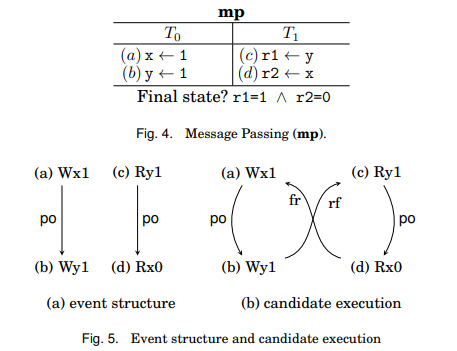
\includegraphics[scale=0.8]{Example_Execution.png}
            }
        \end{figure}


    \end{frame}

    \note{
        Traditionally, axiomatic specification has been proven fruitful for scalable verification of concurrent programs.
        The execution graphs represent a possible execution of the original program.
        These graphs are typically annotated with information that we do have in a program execution.
    }


    \begin{frame}{Core component 2} 

        Critical cycles in execution graphs:
        \begin{itemize}
            \item Minimal cycles that are at least present in an execution graph.
            \item Transitive properties of partial orders in graphs ().
            \item Every model considered at least respects coherence (SC-per location).
        \end{itemize}
        
    \end{frame}


    \begin{frame}
        
        Minimal cycle detection: 
        \begin{itemize}
            \item (MC1) Per thread, at most 2 memory accesses, connected by a direct edge in the cycle.
            \item (MC2) Overall, at most 3 accesses to same memory in the cycle. 
        \end{itemize}

        \begin{figure}
            \makebox[\textwidth][c]{
                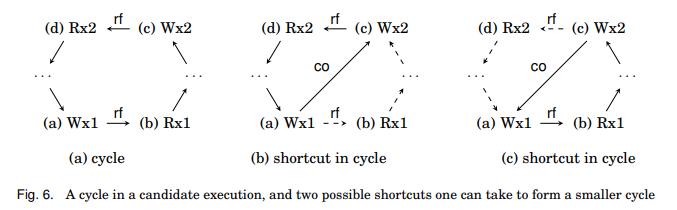
\includegraphics[scale=0.8]{Critical_Cycles.png}
            }
        \end{figure}

    \end{frame}

    \note{
        Minimal cycles are identified using primarily the transitive property of $\po \cup \rf$.
        There is an additional order on memory writes which is not discussed so far in the paper in detail (viz. coherence order $\co$), which is total over accesses on same memory.
        These two orders help us identify minimal cycles, which basically boil down to MC1 and MC2.
        Note that minimal cycles is constrained by length or number of nodes in the cycle. 
    }

    \begin{frame}

        A delay is $\po$ or $\rf$ edge that can cause a weak behavior.
        A behavior is not SC but in weaker model A if and only if 
        \begin{itemize}
            \item (D1) There is at least one cycle with a delay edge.
            \item (D2) All cycles have a delay.
        \end{itemize} 
        
    \end{frame}

    \note{
        A delay is a possible edge that can contribute to a weak behavior.
        In truth, this edge can also not be a delay, pertaining to an execution having a cycle or not.
        Its use is solely in the executions that have cycles.
        This is reminiscent of what we do as crucial reads in an execution.
        
        (D1) is straightforward, as if no delay, the cycle disallows behaviors in both SC and A. 
        (D2) again is based on the same reasoning as D1, as even if one cycle has no delay it is not allowed both in SC and A.
        
        Identifying the delay edges is parametric to the weak memory model A under consideration. 
    }

    \begin{frame}
        
        Critical cycles are minimal cycles which are not allowed in SC but in a weaker model A.
        A cycle is critical for memory model A if and only if 
        \begin{itemize}
            \item (CS1) At least one delay in the cycle.
            \item (CS2) Per thread, at most two accesses, to different locations.
            \item (CS3) There are at most 3 accesses to same memory location.
        \end{itemize}

        nb: Assume all models adhere to coherence (SC-per-location)

    \end{frame}


    \note{
        CS1 is directly from D1.
        CS2, if exists with same location, will violate coherence (go casewise using MC1, MC2, D2).
        CS3 is a little unsure to me too, does not make sense as of now.

    }

    \begin{frame}{Core Component 2}

        Static detection of critical cycles
        \begin{itemize}
            \item Enumerating all executions and testing for cycles will not scale.
            \item Goal is to identify places to insert fences to restore SC.
            \item Instead, map a program to an overapproximation of the program's behaviors, called Abstract Event Graph (aeg).
        \end{itemize}
        
    \end{frame}

    \begin{frame}{From C programs to Goto Equivalents}
        
        Map a C program to an equivalent C program purely with goto statements.
        \begin{itemize}
            \item Replace conditional branching (if statements) with goto equivalents.
            \item Replace loop structure (while/for/do statements) with goto equivalents. 
        \end{itemize}

        \begin{figure}
            \makebox[\textwidth][c]{
                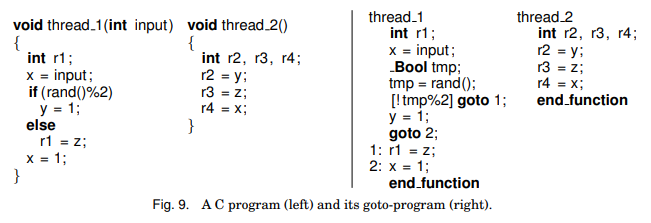
\includegraphics[scale=0.8]{C_Goto_Program.png}
            }
        \end{figure}


    \end{frame}

    \note{
        The choice for converting a program to its goto equivalent is not explained. 
        My guess is that this is rather a choice of convenience in terms of designing the algorithm to derive abstract event graphs.
        Apart from the feasibility of the algorithm, the only other explaination I have is they mention CProver has the same representation of C programs.
        Thus, it could simply be reusability of this mapping already done by CProver, or that they would want to use this tool to extend existing work towards model checking (verification). 
    }

    \begin{frame}{C-goto Program to aeg}

        \begin{itemize}
            \item Extract only the shared memory events, removing local computations.
            \item Retain syntactic order between memory events ($\po_{s}$).
            \item Derive the binary relation relating two events that could cause a data race ($\cmp$)
        \end{itemize}

        \begin{figure}
            \makebox[\textwidth][c]{
                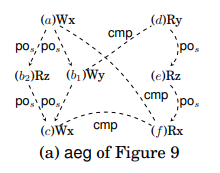
\includegraphics[scale=0.8]{aeg_Example.png}
            }
        \end{figure}

        
    \end{frame}
    
    \note{
        Notice that the read events or write events both do not have concrete values.
        This is reminiscent of our idea on pre-trace model for memory consistency.
        The values are made concrete only while adding $\rf$ and other relations.
        Although what is not clear is the possible write values that a write can have.
        However, note that the aeg does represent all possible candidate executions of the original program.
        This was also proven by them.
    }

    \begin{frame}{aeg to Concrete (candidate) executions}

        \begin{itemize}
            \item Give writes and reads concrete values.
            \item Read concrete values need a write to exist with the same concrete value.
            \item Add $\rf$ edges, and concrete $\po$ edges, taking one control flow path for each branching. 
            \item Lastly, add $\co$ edges.
        \end{itemize}

        \begin{figure}
            \makebox[\textwidth][c]{
                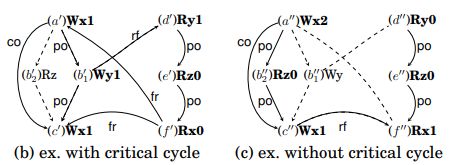
\includegraphics[scale=0.8]{Concrete_Execution.png}
            }
        \end{figure}

        
    \end{frame}

    \note{
        This mapping to candidate executions is very much the same way we map pre-traces to candidate executions.
        The only concern where the difference might be evident is when the branch choice is made, does it depend on the concrete read values or is it also random.
        If it is the former, then there is a clear difference between our model and theirs.
        If it is the latter, then their and our representation may just be the same (perhaps discuss with Clark about this).
    }


    \begin{frame}{Fences and Dependencies}

        \begin{itemize}
            \item Fences are encoded in aeg as special abstract events (nodes) in the graph (eg: mfence in x86).
            \item Dependencies are not part of the aeg, but are recorded.
        \end{itemize}
        
    \end{frame}

    \note{

        The choice of not encoding dependencies into the aeg is not clear to me.
        Perhaps the way to do it would be an edge in the graph, but the edge itself could then complicate our definition of what is a critical cycle and so on.
        Maybe keeping it separate is a good choice, the aeg is much simpler and the dependency calculation can be used separately to determinte fence insertions.

    }

    \begin{frame}{Loops in aeg}

        \begin{itemize}
            \item aeg abstracts away the loop body entirely.
            \item The read/write values are not concrete, thus the loop's behavior is more generalized.
            \item To find critical cycles, a loop body must be duplicated at least once(check CS2), which helps us have edges relating events between any two iterations of the loop.
        \end{itemize}
        
    \end{frame}

    \note{
        This idea is actually very useful and it helps us guarantee that we only need to consider loops as two iterations and nothing more.
        All of this is on the premise that events do not have concrete values.
        I am guessing for infinite loops, this may also be the case.
        But still, have to think on this a bit more.
    }

    \begin{frame}{Critical cycle detection}
        
        \begin{itemize}
            \item Cycle detection done with previous work (Tarjan's Algorithm).
            \item Algorithm finds all elementary circuits in a directed graph.
            \item Complexity is $O((V + E) * (C+1)$, where for vertices (V), edges (E) and circuits (C) in graph.
        \end{itemize}

        \begin{itemize}
            \item Critical cycle detection is done using previous rules. 
        \end{itemize}

    \end{frame}

    \note{
        Honestly, this algorithm can be parallelized too.
        Since their main proponent is to speed up fence insertion to make it scalable for bigger programs, a natural extension would be to change the cycle detection algorithm itself. 
    }


    \begin{frame}{Identifying fence insertions}

        \begin{itemize}
            \item Fence placement is thread-local, between events that partake in a critical cycle and are in the same thread.
            \item Optimal placement depends on how many potential critical cycles can exist in one aeg, with overlapping cycle paths in the same thread.
            \item Placing fences that eliminate most cycles would be the way to go.
            \item However, doing this for multiple threads and assessing is non-trivial. 
            \item To add, there are multiple fence instructions, given different target architectures, each being stronger or weaker than the other.
        \end{itemize}
        
    \end{frame}

    \note{
        The paper delves into different types of fences as well handling cumulativity.
        I think cumulativity is actually pretty non-trivial to address, due to dependencies that must exist accross code fragments.
        I am not sure why they did not just use the dependency calculations done earlier from the program, and use that instead of inserting your own fences again.
        This is okay as they anyways disable compiler optimizations.
        So it should ideally be fine.
    }

    \begin{frame}{Optimizing fence insertions (ILP)}

        \begin{itemize}
            \item Frame the minimization of fences as an ILP.
            \item Associate each fence with a cost and calculate the minimization
        \end{itemize}

        \begin{figure}
            \makebox[\textwidth][c]{
                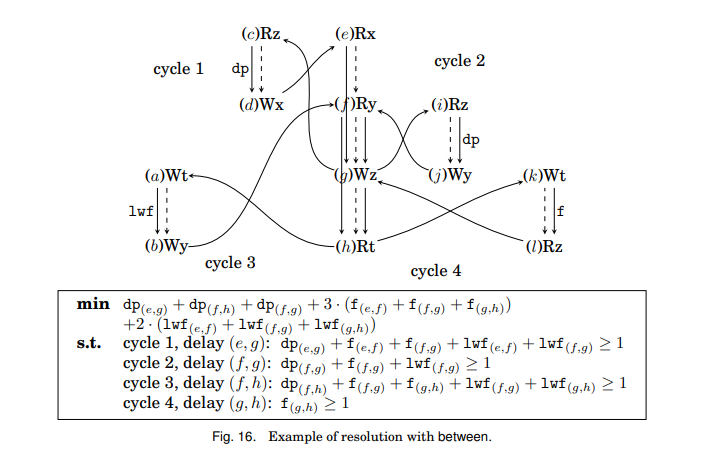
\includegraphics[scale=0.6]{Fence_Insertion.png}
            }
        \end{figure}

    \end{frame}

    \note{ 
        This is a very smart solution to address the minimization problem.
        However, it turns out to be suboptimal which is observed in the testing phase.
        I am not sure why it is suboptimal, and perhaps a solution to it might lead to a good publication (talk with Clark, reel in someone else I guess?).

    }

    \begin{frame}{Actual fence/dependency placement}

        \begin{itemize}
            \item Fences are inserted into C code as inline assembly (why I wonder).
            \item Dependencies require some more work to just introduce a dependency (again via inline assembly) in the code.
        \end{itemize}

        \begin{figure}
            \makebox[\textwidth][c]{
                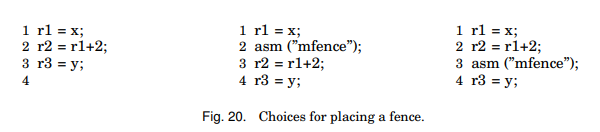
\includegraphics[scale=0.8]{Fence_Placement.png}
            }
        \end{figure}

        
    \end{frame}

    \begin{frame}{Testing, comparing with other techniques}
        
        \begin{itemize}
            \item Testing how much time it takes to identify fence placements.
            \item Testing how many fences are to be added. 
        \end{itemize}

        \begin{figure}
            \makebox[\textwidth][c]{
                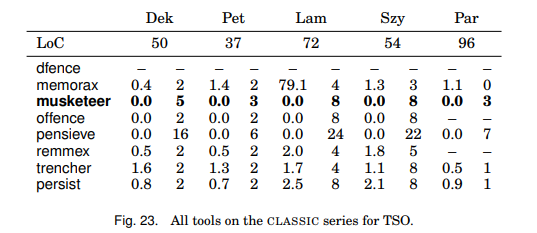
\includegraphics[scale=0.8]{Time_NFences.png}
            }
        \end{figure}

    \end{frame}

    \begin{frame}

        \begin{itemize}
            \item Testing runtime overheads due to placement of fences (M is the proposed implementation).
        \end{itemize}

        \begin{figure}
            \makebox[\textwidth][c]{
                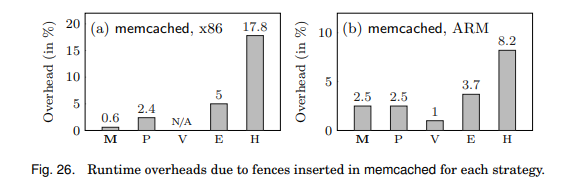
\includegraphics[scale=0.8]{Runtime_Overhead.png}
            }
        \end{figure}

    \end{frame}

    \note{

        It is interesting to note that while fences suggested to add is more in some cases for musketeer, it still shows relatively less overhead.
        Perhaps the cases for which additional fences were suggested, the case is not covered in the bigger examples of Debian packages.

    }

    \begin{frame}{Conclusion}
        
        \begin{itemize}
            \item Fence insertion techniques not scalable.
            \item Propose a new technique which statically determines fence placements.
            \item Relies on overapproximation of program behavior, using abstract event graphs.
            \item Framed minimal fence insertion as an ILP problem.
        \end{itemize}

    \end{frame}

\end{document}